\section{Methods}\label{sec:methods}

\subsection{Dataset}

The data used for this paper originates from the 'Monitoring error-related potentials' dataset, which was created by {INSERT REF} et al. This dataset is publically available on the BCNI Horizon 2020 project website. In this dataset, users were placed in front of a screen where they had to observe a moving cursor. The working area of the screen consisted of 20 locations along the horizontal plane. A coloured square would appear either on the cursor's left or right and indicate the target to which the cursor should move. The cursor would move along the horizontal axis towards the target at each trial. Once the target has been reached, the cursor will stay in place, and a new target will appear along the horizontal plane, no more than three positions away from the cursor.

During the experiments, users were asked to solely monitor the agent's performance, knowing the goal of reaching the target. They had no control over the cursor. At each trial, there was a 20\% chance for the cursor to move in the opposite direction relative to the target, which contradicts the agent's goal. These trials are labelled as 'Error-related potentials.'

Six users participated in this experiment, each performing two separate recording sessions. Each session consisted of 10 blocks, of 3 minutes each. Each trial consisted of approximately 50 trials. The EEG signals were recorded at a sampling rate of 512hz.

Since the users have no control over the cursor, the task is purely mental. This results in fewer signals originating from the motor complex being present in the EEG. However, the lack of physical movements also makes it easier for participants to lose focus and start mind wandering. This would inevitably result in more unwanted signals creeping into the EEG.


\subsection{Preprocessing}

\subsubsection{Filtering}

EEG data is very prone to noise originating the environment. One such example is the frequencies originating from the power-line, which are 50 hz. To reduce this noise the raw data is being fed through a butterworth filter with a low-pass of 1hz, and a high pass of 10hz.

\subsubsection{Epoching}

The used dataset contained six different labels for trials. Two of those labels indicate that the cursor moved towards the target, which will be labeled as a 'non error-related potential'. Two other labels indicate that the cursor moved in the opposite direction compared to the target. These are labeled as 'error-related potentials'.These two labels will furtheron be referred to as \verb|ErrP| and \verb|non-ErrP| signals. The two remaining raw labels are ignored.

\begin{figure}[!tbp]
    \centering
        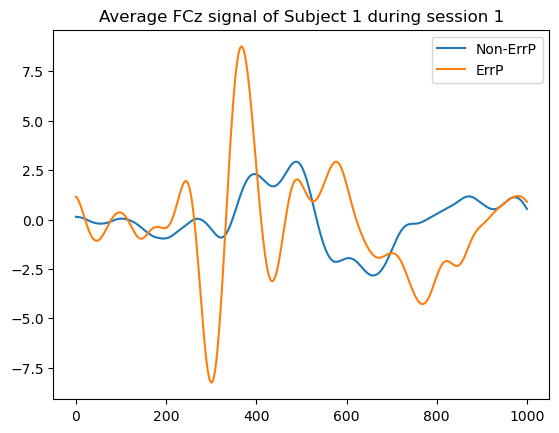
\includegraphics[width=7.7cm]{img/FcZs1s1-1000ms.png}
    \caption{Graph of the average non-ErrP and ErrP signal in the FcZ channel. These signals originate from subject 1 during session.}
    \label{fig:FcZ}
\end{figure}

Figure \ref{fig:FcZ} shows that the largest difference between \verb|ErrP| and \verb|non-ErrP| signals occur between 200 and 500 milliseconds after the feedback presentation. For this reason, the window size will be made 600ms, to capture these differences between signals. Note that this graph only shows the FcZ channel, but this channel is the most prominent for ErrP signals.

This resulted in the input EEG data being a matrix of size 64 x 308. Where the number of rows are the 64 channels of the EEG, and the number of columns are the length of the windows, 600ms of 512hz sampling rate.

The dicision of feeding al 64 channels into the model was made because of two reasons. First, previous experiments {INSERT REF} have shown that feeding all channels, as opposed to pre-selecting electrodes, resulted in consistently better accuracy. Second, the main aim of this research is to study uncertainty. Having all channels could present more interesting results with regard to the amount and origin of uncertainty, as opposed to only using a select amount of channels.

\subsubsection{Balancing}

Due to the nature of the experiment of the used dataset, the data is inherently unbalanced with a 1/5 ratio. Only 20\% of the trials are \verb|ErrP| trials. Rebalancing is necessary to prevent the model from predicting all input episodes as \verb|non-ErrP|. To achieve this, in the training set, the under-represented class \verb|ErrP| will be over-sampled until the two classes are represented equally.

To stick as close as possible to the real-world application of these classifiers, the dataset split for the training, validation and testing of the model was carefully considered. One participant is put aside for the testing set, and the remaining five participants will be used for training. Furthermore, 20 trials are randomly sampled from the training set to be used as a validation set. This results in approximately 66.7\% of the data being used for training, 16.7\% for validation, and 16.7\% for testing, with the latter being a participant the model has not yet seen in training and validation. 


\subsection{Model}

\subsubsection{Model architecture}

The main body of the model architecture consists of a model called EEGNet, a compact convolutional network tailored explicitly for BCI EEG classification {INSERT REF}. This model consists of two distinct sequential blocks. 

The first block consists of two convolutional steps in sequence. The first layer applies $F_1$ convolutional filters of size (1, 64), which capture the EEG signal at different band-pass frequencies. Setting $F_1$ to half the sampling rate allows for capturing frequency information at 2Hz and above. Next, a \verb|Depthwise Convolution| is applied to learn a spatial filter. After each convolutional layer, batch normalization is applied. Next, an exponential linear unit (ELU) is applied, followed by a Dropout layer to help regularize the model. Lastly, an average pooling layer is used to reduce the sampling rate to a quarter of the original sampling rate.

The second block consists of a Separable Convolution, which is a Depthwise Convolution followed by $F_2$ Pointwise Convolutions. These convolutions help reduce the number of parameters to fit and explicitly decouple the relationship across feature maps. This operation separates the learning of how to summarize individual feature maps in time from how to combine these feature maps optimally. An Average Pooling Layer follows this block to reduce the free parameters in the model.

In the original model, inputs are passed through the two blocks sequentially, followed by a flattened layer. This is followed by a linear layer, which gives the logits of the model's prediction. This output layer is where our model differs from the original mode. Rather than having only one layer returning the classification logits, our model uses two output layers called \verb|heads|. The first head is a linear layer returning the logits representing the \verb|mean| of the prediction. The second head is a linear layer followed by a softplus. This head returns logits representing the \verb|variance| of the model. The softplus is necessary to make the variance positive.


\subsubsection{Sampling softmax}

The goal is to capture heteroscedastic aleatoric uncertainty in the model. Currently, our model predicts two tensors. One contains the prediction of the mean of both classes. The other contains the prediction of the variance of both classes. To achieve this capture of heteroscedastic aleatoric uncertainty, a gaussian distribution is placed over the unaries.

\begin{equation}
    \hat{x}|w \sim \mathcal{N}(f^w, (\sigma^w)^2)
\end{equation}

\begin{equation}
    \hat{p} = Softmax(\hat{x})
\end{equation}

Here, $f^w$ is the output of mean head with parameters $w$. $\sigma^w$ is the output of the variance head with parameters $w$. The prediction consists of $f^w$, which is corrupted with Gaussian noise with a variance of $\sigma^w$. The corrupted vector is then squashed with the Softmax function to obtain a vector of probabilities.

Ideally, an analytical integral should be taken from this Gaussian Distribution. However, no such solution exists to achieve this. Therefore, an approximation of the integral has to be made. This is achieved through Monte Carlo integration. Here we sample from the aforementioned normal distribution, and apply the softmax function to each sample. Using these samples, we can calculate the mean and variance.


\subsubsection{Loss function}

This raises a question. How can we find the optimal model parameters $\theta$, which results in the most accurate predictions of the mean, while simulatinously predicting a variance capturing the aleatoric uncertainty? The loss function should allow the model to reduce the received loss by predicting a high variance on incorrect predictions. However, it is undesirable if the model predicts high variance on all input sequences, and thus needs to be punished for predicting high uncertainty on correct predictions. One may ask how this can be achieved. Previous research by {INSERT REF} found such method to achieve this desired behavior. This method is called $\beta$-NLL.

\begin{equation}
    \mathcal{L}_{\beta-NLL} := \sum_{i = 1}^{n} \left( \lfloor \hat{\sigma}^{2\beta}(X) \rfloor NLL \right)
\end{equation}

Here, the $\lfloor. \rfloor$ indicates the \verb|stop gradient| operator. This makes $\hat{\sigma}^{2\beta}(X)$ act as a learning rate, which is dependant on the variance prediction. If $\beta$ is set to a value of 0, the loss function behaves like a normal NLL loss. If the value is set to $0.5$, interesting behaviour is observed. Now, all data points are weighted down by $\frac{1}{\sigma}$ (inverse standard deviation instead of inverse variance). Experiments conducted by {INSERT REF}, showed that $\beta = 0.5$ achieved the best balance between accuracy and log-likelihood.

To find the optimal parameters $\theta$, the negative log-likelihood (NLL) is used:

\begin{equation}
    NLL := \frac{1}{2}\log \hat{\sigma}^2(X) + \frac{\mathcal{L}_\theta}{\hat{\sigma}^2(X)}
\end{equation}

This loss measures the decrepancy between the predicted distribution and the target distribution, assuming a Gaussian distribution with mean $\mu$ and variance $\sigma^2$. Here, the left term $\frac{1}{2}\log \hat{\sigma}^2(X)$ acts as a normalization factor for the NLL loss, which ensures the model learns to predict the best possible mean and variance parameters for the given data. In the right term, $\mathcal{L}_\theta$, is the loss function used nested in the NLL loss. This loss is divided by $\hat{\sigma}^2(X)$. By dividing thiss loss by the variance, we ensure that the NLL loss is sensitive to both the accuracy of the predicted mean $\mu$, and the uncertainty estimation encoded in the predicted variance $\sigma^2$. A higher uncertainty estimation, results in a higher dividing factor, and thus a lower loss. The first term ensures the model doesn't always predict a high $\sigma^2$.

In the original paper, the task at hand was a regression task, and the used loss function $\mathcal{L}_\theta$ was the mean squared error loss (MSE). In our case, the task at hand is a classification task. For this, we will use the Binary Cross Entropy loss (BCE):

\begin{equation}
    \mathcal{L}_\theta := - ( Y \log \hat{\mu}(X) + (1 - Y) \log (1 - \hat{\mu}(X)) )
\end{equation}

The BCE loss measures the difference between the predicted probability distribution of the binary output variable, and the true probability distribution of said variable. The first term in this function, $Y \log \hat{\mu}(X)$, punishes the model when it predicts a low probability $\mu(X)$ for the positive class. Similarely, the second term punished the model when it predicts a high probability for the negative class. Together, these two terms ensure that BCE loss penalizes the model for making incorrect predictions.

The combination of these three elements, allow $\beta$-NLL to ensure that the model learns to predict an optimal mean $\mu$, and a variance $\sigma^2$, capturing the aleatoric uncertainty of the model.


\subsection{Explainable AI}

To be able to understand what our model is doing, and explain where the uncertainty is originating from, we need to introduce a method of Explainable AI to our model. For this, a method based on shapley values will be used.

Shapley values are a concept which originate from the field of cooperative game theory. They provide a way of allocating a value generated by a group of players to each individual player. This strategy has been widely adapted to the field of machine learning. Here, they attribute the contribution of each individual input feature to the final prediction of the model. This resulting attribution method is called SHAP (SHapley Addaptive exPlanations)

The key idea behind SHAP values is to decompose the model's output into the contribution of each input feature, while also taking into account their relations with the other features. Exact calculations are practically impossible to calculate for larger inputs. Instead, the SHAP values are calculated by approximation. This algorithm involves sampling a subset of the features, and computing the SHAP values for each sample. The final values are then averaged over all samples to obtain an estimate of the feature importance.

The advantage of using the SHAP approach, is its flexibility and generality. They can be applied to a wide range of models, including classification tasks. Moreover, they provide a rich and interpretable representation of the model's behaviour. Another advantage of SHAP values, is that we can differentiate between the two heads. Using SHAP, we can build understanding of how each feature contributed solely to the mean prediction. And how they contributed solely to the variance prediction. The latter being of extreme interest in explaining the origins of the uncertainty. 

\subsection{Experiment design}

